\chapter{Marco Referencial}
\label{cap:marco}

El Capítulo~\ref{cap:generalidades} planteó el problema y los objetivos en
términos del dominio: grabaciones, anotaciones y tiempo de especialista. Este
capítulo fija los conceptos que esos objetivos dan por sentados. El marco teórico
formaliza la tarea como detección de eventos sobre el espectrograma y precisa qué
significa predecir una caja tiempo--frecuencia. El marco conceptual define los
términos que los capítulos de resultados usan sin volver a explicarlos: paisaje
sonoro, evento acústico, representación tiempo--frecuencia, detección de eventos
sonoros, clasificación jerárquica y anotación inconsistente.

\section{Marco Teórico}

\subsection{Formulación del problema de detección}
\label{sec:formulacion}

El problema se plantea en dos niveles. El nivel de la \emph{grabación} es el que
le interesa al analista y define el producto; el nivel de la \emph{ventana} es el
que consume el modelo y define su entrada y su salida. Separarlos es necesario
porque ninguna arquitectura actual procesa una hora de audio de una sola vez, y
confundirlos oscurece qué predice realmente un detector.

\paragraph{Nivel de grabación}
El sistema recibe un conjunto de grabaciones $G=\{g_1,g_2,\dots,g_M\}$. Cada
grabación $g_k$ es una señal de audio $x(t)$ en formato WAV, muestreada a
$F_s = 44{,}1$\,kHz, de duración $D_k$ que puede llegar a la hora. Para cada una
el sistema debe devolver una lista de eventos $E_k=\{e_1,e_2,\dots,e_{N_k}\}$,
cuyo cardinal $N_k$ no se conoce de antemano y donde cada evento es la tupla

\begin{equation}
    e_i = \bigl(t^{(i)}_{\text{ini}},\; t^{(i)}_{\text{fin}},\;
    f^{(i)}_{\min},\; f^{(i)}_{\max},\;
    y^{(i)},\; p^{(i)}\bigr).
    \label{eq:tupla}
\end{equation}

\begin{description}
    \item[$(t_{\text{ini}}, t_{\text{fin}})$] Instantes de inicio y fin del
          evento, en segundos desde el comienzo de la grabación, con
          $0 \le t_{\text{ini}} < t_{\text{fin}} \le D_k$.

    \item[$(f_{\min}, f_{\max})$] Banda de frecuencia que ocupa el evento, en
          hercios, con $0 \le f_{\min} < f_{\max} \le F_s/2$. Es la componente que
          distingue esta formulación de la detección de eventos sonoros puramente
          temporal.

    \item[$y$] Etiqueta tomada de un vocabulario cerrado
          $Y=\{y_1,\dots,y_L\}$ cuyos elementos son pares de especie y tipo de
          llamada. La sección~\ref{sec:etiqueta} justifica por qué la etiqueta es un
          par plano y no dos niveles predichos por separado; las proyecciones
          $\pi_{\text{esp}}(y)$ y $\pi_{\text{tipo}}(y)$ recuperan cada nivel cuando
          se lo necesita.

    \item[$p$] Confianza en $[0, 1]$ asignada por el modelo, que ordena las
          predicciones y define el punto de operación de la revisión asistida.
\end{description}

Las cuatro primeras componentes definen una caja rectangular sobre el plano
tiempo--frecuencia, la misma que el especialista dibuja en Raven
(Figura~\ref{fig:annotation-example}); las dos restantes la etiquetan y la
puntúan.

\paragraph{Nivel de ventana}
La grabación se recorta en ventanas de duración fija $T_w$, tomadas cada $H$
segundos con $H < T_w$, de modo que ningún evento quede siempre partido por un
borde. Cada ventana se convierte en un espectrograma mel
$X \in \mathbb{R}^{F \times T}$, con $F$ bandas de frecuencia y $T$ tramas
temporales, y ese tensor es la entrada del modelo.

El detector es una función de parámetros $\theta$ que a cada ventana le asigna un
conjunto de tamaño fijo

\begin{equation}
    f_\theta(X) = \bigl\{(\hat{b}_q,\; \hat{\pi}_q)\bigr\}_{q=1}^{Q},
    \qquad
    \hat{b}_q \in [0, 1]^4,
    \qquad
    \hat{\pi}_q \in [0, 1]^{L+1},
    \label{eq:modelo}
\end{equation}

donde $Q$ es un número de consultas fijado por la arquitectura, independiente del
contenido de la ventana y mayor que la cantidad de eventos que cabe esperar en
ella. Cada consulta produce una caja $\hat{b}_q = (c_x, c_y, w, h)$ en
coordenadas normalizadas al recuadro de la ventana (centro, ancho y alto, los
cuatro en $[0, 1]$) y una distribución $\hat{\pi}_q$ sobre
$Y \cup \{\varnothing\}$, en la que $\varnothing$ es la clase ``sin objeto'' que
absorbe las consultas sobrantes. El número de eventos no se predice: resulta de
cuántas consultas eligen una clase de $Y$ por encima del umbral de confianza.

Esta es la formulación de \emph{predicción de conjuntos}: la salida no es una
rejilla puntuada ni una secuencia, sino un conjunto sin orden, y durante el
entrenamiento cada anotación de la ventana se asigna a exactamente una consulta
mediante un emparejamiento biyectivo, mientras que el resto se supervisa hacia
$\varnothing$. De ahí que dentro de la ventana no haya anclas ni supresión de no
máximos.

\paragraph{Del marco normalizado al marco físico}
Lo que emite el modelo no son segundos ni hercios sino fracciones de la ventana,
y la conversión no es simétrica entre los dos ejes. En tiempo es afín: si la
ventana empieza en $t_0$,
\begin{equation}
    t_{\text{ini}} = t_0 + \bigl(c_x - \tfrac{w}{2}\bigr) T_w,
    \qquad
    t_{\text{fin}} = t_0 + \bigl(c_x + \tfrac{w}{2}\bigr) T_w.
\end{equation}
En frecuencia no lo es, porque el eje vertical del espectrograma está en escala
mel. Con $m(\cdot)$ la función que convierte hercios a mel y $[f_{\text{lo}},
            f_{\text{hi}}]$ los extremos del banco de filtros, la coordenada normalizada
$u \in [0, 1]$ vuelve a hercios mediante
\begin{equation}
    \varphi(u) = m^{-1}\!\bigl(m(f_{\text{lo}}) + u\,[\,m(f_{\text{hi}}) -
            m(f_{\text{lo}})\,]\bigr),
    \label{eq:mel-inv}
\end{equation}
y entonces $f_{\min} = \varphi(c_y - h/2)$ y $f_{\max} = \varphi(c_y + h/2)$. La
consecuencia práctica es que una caja de altura constante en el marco normalizado
cubre una banda mucho más ancha en la parte alta del espectro que en la baja.

\paragraph{De las ventanas a la grabación}
Como las ventanas se solapan, una misma vocalización puede predecirse en dos o
tres de ellas, y una vocalización más larga que $T_w$ solo puede predecirse por
partes. Las predicciones de toda la grabación se llevan al marco común, se
agrupan por clase y se depuran por supresión de no máximos, de modo que la lista
$E_k$ contenga un evento por vocalización. Ese es el punto en el que el nivel de
ventana devuelve el control al nivel de grabación, y también el punto en el que
el ventaneo deja su huella sobre los eventos más largos que la ventana.

\subsection{El espectrograma y la asimetría de sus ejes}
\label{sec:stft}

La señal de audio es unidimensional, pero los eventos de interés se distinguen
por cómo se distribuye su energía entre frecuencias a lo largo del tiempo. La
transformada de Fourier de tiempo corto (STFT) recupera esa estructura: divide
la señal en tramas solapadas, aplica una ventana a cada una y calcula su
espectro. La magnitud del resultado es el espectrograma, una matriz
$X \in \mathbb{R}^{F\times T}$ cuyos parámetros, como el tamaño de ventana, el salto
entre ventanas y el tipo de ventana, fijan el compromiso entre resolución
temporal y resolución frecuencial.

Interesa aquí una asimetría del espectrograma que conviene explicitar porque condiciona el
diseño del detector. Tratarlo como una imagen es útil, pero sus dos ejes no son
equivalentes: una traslación en tiempo preserva el significado del patrón,
mientras que una traslación en frecuencia lo cambia: un mismo contorno
desplazado media octava es otra vocalización, o ninguna. Los patrones
espectro-temporales de los eventos sonoros dependen de la banda de frecuencia en
que ocurren, de modo que la convolución bidimensional estándar, equivariante a
traslación en ambos ejes, no es adecuada para el eje frecuencial
\citep{nam_frequency_2022}. La consecuencia práctica es que el modelo debe
conservar de forma explícita la posición en frecuencia en lugar de descartarla.

\subsection{Detección de objetos sobre audio}
\label{sec:objetos}

Una vez que el sonido se representa como una matriz tiempo--frecuencia, la tarea
de la ecuación~\eqref{eq:tupla} coincide con la de la detección de objetos en
visión por computadora: afirmar que una clase está presente y localizarla,
localización que se representa típicamente mediante una caja delimitadora
\citep{lin_2014}. La analogía no es superficial. Los eventos acústicos se
manifiestan como patrones bidimensionales de tiempo y frecuencia, con texturas y
estructuras geométricas propias, análogos a los objetos que aparecen en imágenes
naturales \citep{pham_eventness_2018}, y el encuadre trasciende la bioacústica
hacia el análisis de señales en general \citep{wood_deep_2022}.

\rotulo{Familia R-CNN.} Los detectores de dos etapas proponen primero regiones
candidatas y luego las clasifican y refinan. Sobre espectrogramas, un detector de
dos etapas localiza llamadas de aves migratorias nocturnas \citep{airale_nbm_2025},
y DeepSqueak, construido sobre Faster R-CNN, se ha usado con las vocalizaciones de
un primate en cautiverio \citep{romero-mujalli_utilizing_2021}.

\rotulo{Familia YOLO.} Los detectores de una etapa, cuyo representante más
difundido es YOLO (\textit{You Only Look Once}), predicen clase y caja en una
sola pasada sobre una rejilla, lo que los hace más rápidos y más simples de
entrenar. Su uso sobre espectrogramas está reportado como línea base competitiva
\citep{gonzalez_yolo-based_2025}, y YOLOv5 se ha aplicado a vocalizaciones de
foca barbuda \citep{escobar-amado_computer_2024}. La misma idea de una sola
pasada inspira a YOHO, que la aplica al eje temporal \citep{venkatesh_you_2022}.

\rotulo{Familia DETR y transformadores.} Los detectores basados en atención
eliminan las anclas y la supresión de no máximos, y formulan la detección como
la predicción directa de un conjunto de objetos emparejado con las anotaciones.
Su adaptación al audio es reciente: SoundDet trata el audio crudo como una señal
espacio-temporal y detecta eventos móviles sobre ella \citep{he_sounddet_2021}, y
\citet{zhu_sound_2025} combinan un transformador de espectrograma autosupervisado
con un decodificador deformable de esta familia para detectar cajas
tiempo--frecuencia, el precedente directo de la arquitectura propuesta en esta
tesis.

\rotulo{Cajas frente a máscaras.} Una alternativa a la caja es la segmentación
semántica, que asigna una etiqueta a cada celda tiempo--frecuencia y describe
con más fidelidad los contornos de una vocalización \citep{jin_semantic_2022}.
Esta tesis opta por la caja por dos razones: es la forma en que el analista
anota en Raven, y por tanto la única para la que existe una referencia
disponible; y es la que se exporta sin pérdida a una tabla de selección. Una
máscara exigiría reanotar el corpus completo.

\section{Marco Conceptual}

Los conceptos que siguen no se presentan por área temática sino siguiendo el
recorrido de la señal, desde que el animal vocaliza hasta que el analista recibe
una etiqueta revisable. La Figura~\ref{fig:signal-chain} dibuja ese recorrido
como una cadena de seis eslabones.

\begin{figure}[htbp]
    \centering
    \caption{Cadena de la señal}
    \label{fig:signal-chain}
    \resizebox{\textwidth}{!}{%
        \begin{tikzpicture}[
                every node/.style={font=\footnotesize},
                eslabon/.style={caja, draw=azul!70, fill=azul!6, align=center,
                        text width=26mm, minimum height=15mm, inner sep=3pt},
                perdida/.style={font=\scriptsize, text=rosa!75!black, align=center,
                        text width=27mm},
                paso/.style={-{Stealth[length=2.2mm]}, thick, draw=azul!70},
            ]
            \node[eslabon] (v) {\textbf{Vocalización}\\[1pt]
                {\scriptsize el aparato fonador fija la banda de frecuencia}};
            \node[eslabon, right=5mm of v] (p) {\textbf{Propagación}\\[1pt]
                {\scriptsize atenuación con la distancia, enmascaramiento del coro}};
            \node[eslabon, right=5mm of p] (g) {\textbf{Grabadora}\\[1pt]
                {\scriptsize AudioMoth, 44,1\,kHz, mono}};
            \node[eslabon, right=5mm of g] (s) {\textbf{STFT}\\[1pt]
                {\scriptsize ventana 1024 (23\,ms), salto 400 (9\,ms)}};
            \node[eslabon, right=5mm of s] (m) {\textbf{Mel + compresión}\\[1pt]
                {\scriptsize 128 bandas HTK, 25\,Hz--22,05\,kHz}};
            \node[eslabon, right=5mm of m] (c) {\textbf{Caja anotada}\\[1pt]
                {\scriptsize cuatro coordenadas y dos etiquetas}};
            \foreach \a/\b in {v/p, p/g, g/s, s/m, m/c}
            \draw[paso] (\a) -- (\b);
            \node[perdida, below=4mm of p] {pierde relación señal-ruido, sobre todo en agudos};
            \node[perdida, below=4mm of g] {pierde lo que supera 22,05\,kHz};
            \node[perdida, below=4mm of s] {compromiso entre tiempo y frecuencia};
            \node[perdida, below=4mm of m] {resolución no uniforme};
            \node[perdida, below=4mm of c] {un rectángulo aproxima un contorno};
        \end{tikzpicture}}
\end{figure}

Debajo de cada eslabón figura lo que se pierde en él: la propagación resta
relación señal-ruido, sobre todo en los agudos; la grabadora descarta lo que
supera 22,05\,kHz; la STFT obliga a elegir entre resolución temporal y frecuencial;
la escala mel reparte la resolución de forma no uniforme, y la caja aproxima con
un rectángulo un contorno que no lo es. Cada pérdida crea la necesidad del
eslabón siguiente, y por eso las subsecciones siguen el orden en que aparecen los
problemas.

\subsection{Paisaje sonoro}

La bioacústica estudia el sonido en los seres vivos, y esta tesis la aplica a
través del monitoreo acústico pasivo descrito en la sección~\ref{sec:problema}. Lo
que la grabadora registra no es la vocalización sino la suma de todo lo que llega
al micrófono, el paisaje sonoro del ecosistema \citep{blumstein_acoustic_2011}, y
en un entorno como la Amazonía esa suma tiene tres componentes:

\begin{description}
    \item[Biofonía.] Los sonidos de origen biológico. Incluye la señal de interés,
          las vocalizaciones de primates, y también el coro de insectos, anfibios
          y aves, que ocupa las mismas bandas durante horas seguidas.

    \item[Geofonía.] Los sonidos de origen físico: viento, lluvia, movimiento de
          la vegetación. Su energía se reparte sobre bandas amplias y su carácter es
          o bien cuasi-estacionario o bien de ráfaga.

    \item[Antropofonía.] Los sonidos de origen humano: motosierras, disparos,
          motores. No solo interfieren con la señal, sino que son en sí mismos un
          indicador de presión sobre el ecosistema \citep{blumstein_acoustic_2011}.
\end{description}

A ello se suma la atenuación: el animal está a una distancia desconocida del
sensor, de modo que la misma vocalización llega unas veces nítida y otras apenas
por encima del fondo. El archivo resultante contiene, entonces, una señal
mezclada, atenuada y de relación señal-ruido variable dentro de una misma
grabación. La pregunta que abre el eslabón siguiente es qué hay que buscar dentro
de esa mezcla, es decir, qué constituye exactamente un evento.

\subsection{Eventos acústicos}

La vocalización se produce por el flujo de aire desde los pulmones, que hace
vibrar las cuerdas vocales en la laringe y actúa como fuente sonora primaria; el
tracto vocal supralaríngeo, formado por la faringe y las cavidades oral y nasal,
filtra esa fuente y fija sus características finales: frecuencia fundamental,
distribución de armónicos, amplitud, duración y timbre. Es la teoría
fuente--filtro, que la investigación sobre comunicación vocal de mamíferos aplica
de forma general \citep{taylor_contribution_2010}.

La consecuencia de esa estructura fuente--filtro es la que interesa aquí. La
frecuencia fundamental queda determinada por la geometría y la tensión de las
cuerdas vocales, y las resonancias del tracto vocal concentran la energía en un
conjunto acotado de bandas. Un evento no es, por tanto, un instante con una
etiqueta: es una región del plano tiempo--frecuencia con un límite inferior y un
límite superior de frecuencia que dependen de la anatomía de quien vocaliza. La
banda que ocupa una especie es una propiedad física de su aparato fonador, no una
convención de dibujo del anotador. Esa es la razón por la que la caja
tiempo--frecuencia de la ecuación~\eqref{eq:tupla} es la representación adecuada
del evento, y no un rectángulo elegido por comodidad: los cuatro números que la
definen tienen referente físico.

La misma estructura explica dos hechos que reaparecen más adelante. El primero es
que distintas especies tienden a separarse por banda, lo que hace de la
frecuencia una característica discriminante y no un dato accesorio. El segundo es
que la estructura de las vocalizaciones de los primates no humanos está muy
conservada dentro de cada especie, pero admite ajustes dentro de esos límites,
como los rasgos propios de cada grupo \citep{fischer_towards_2020}; esa
variabilidad amplía el rango de formas que el detector debe reconocer como la
misma clase.

El evento existe, entonces, como región bidimensional. El problema es que la
señal grabada es unidimensional: hay que recuperar esa estructura antes de poder
buscarla.

\subsection{Representaciones tiempo--frecuencia}
\label{sec:frontends}

La STFT, descrita en la sección~\ref{sec:stft}, recupera la dimensión que falta.
Sobre la matriz que produce se aplican dos transformaciones habituales: la escala
mel, que reagrupa las bandas según una progresión aproximadamente logarítmica, y
la compresión logarítmica de la magnitud a decibelios. El resultado, el
espectrograma log-mel, es la entrada estándar en detección de eventos sonoros, y
es la transformación que convierte un problema de audio en uno de análisis de
imágenes.

Ninguno de esos pasos es gratuito. El primero es la longitud de la trama de la
STFT, que fija un compromiso entre las dos resoluciones: la
Figura~\ref{fig:stft-tradeoff} pinta la misma secuencia de sílabas del tamarino
de Weddell con tres longitudes de trama.

\begin{figure}[htbp]
    \centering
    \caption{Compromiso de la STFT}
    \label{fig:stft-tradeoff}
    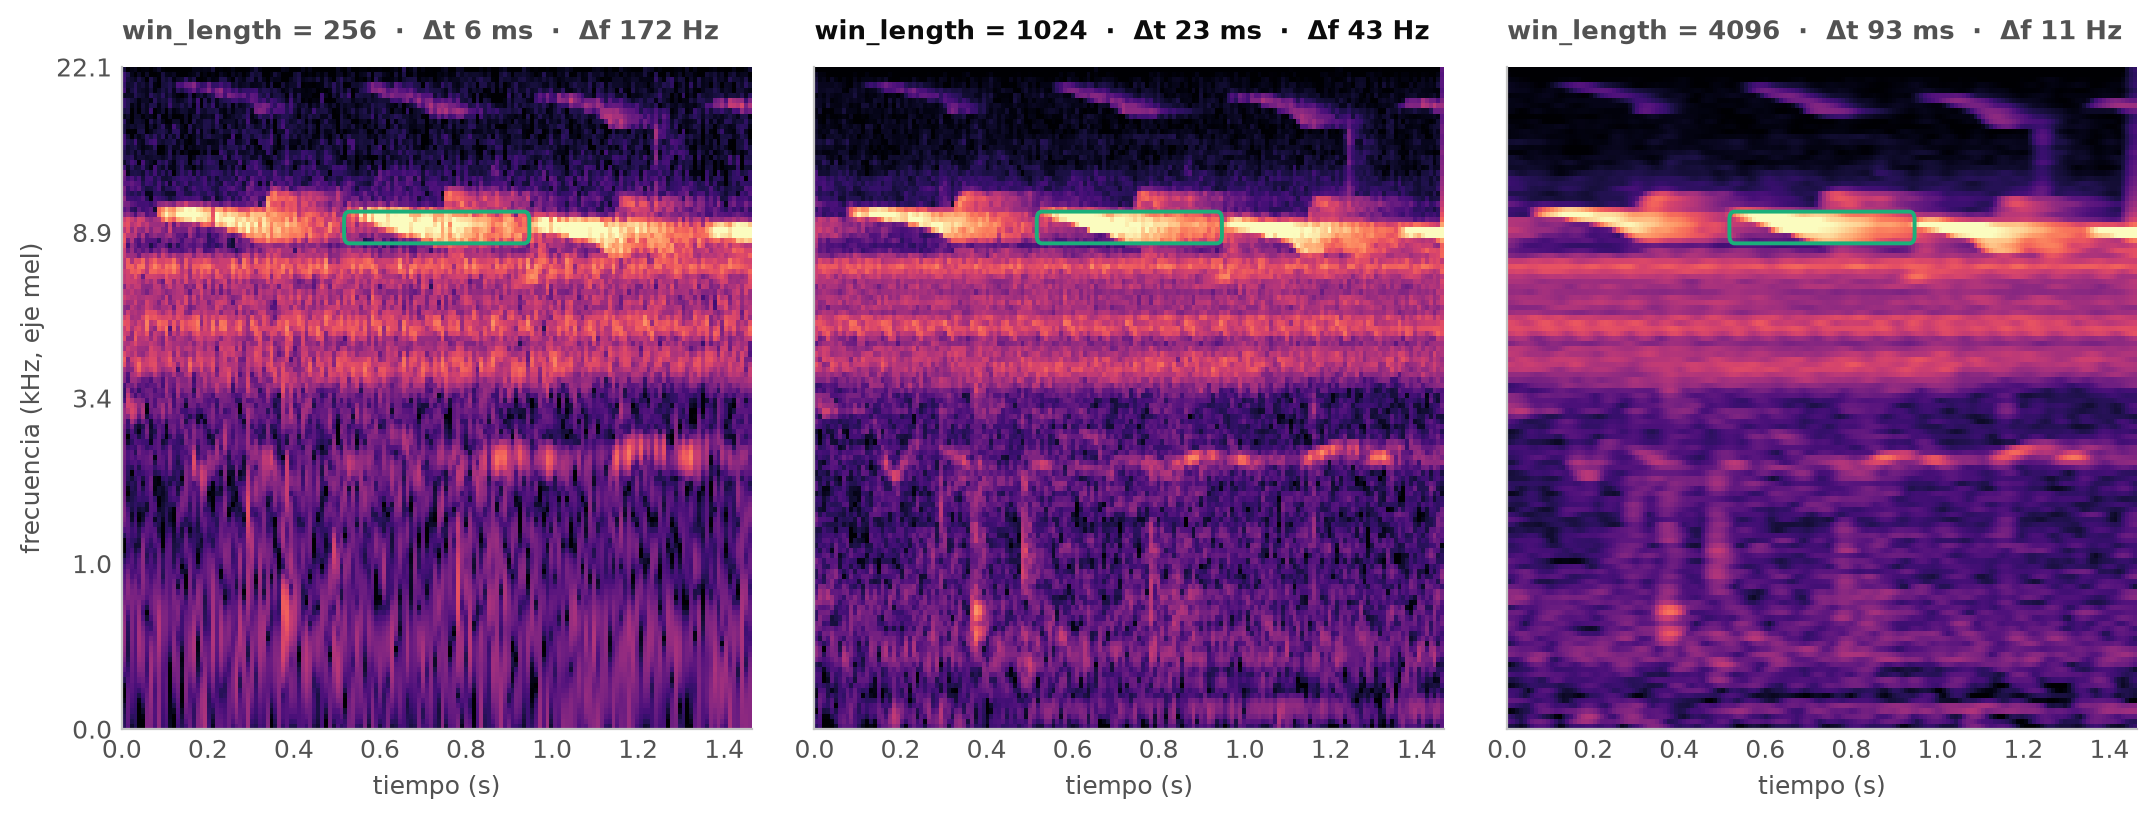
\includegraphics[width=\textwidth]{capitulos/02_marco_referencial/figures/stft_tradeoff.png}
\end{figure}

Con la trama más corta (256 muestras, 6\,ms) cada sílaba queda nítida en el
tiempo pero se emborrona en frecuencia, con una resolución de 172\,Hz; con la más
larga (4096 muestras, 93\,ms) ocurre lo contrario, y los bordes de inicio y fin se
difuminan. La trama intermedia de 1024 muestras, la que usa esta tesis, conserva a
la vez el contorno de la sílaba y sus fronteras.

El segundo paso es la escala mel, que reparte la resolución de forma no uniforme
entre graves y agudos (Figura~\ref{fig:mel-axis}).

\begin{figure}[htbp]
    \centering
    \caption{Escala mel}
    \label{fig:mel-axis}
    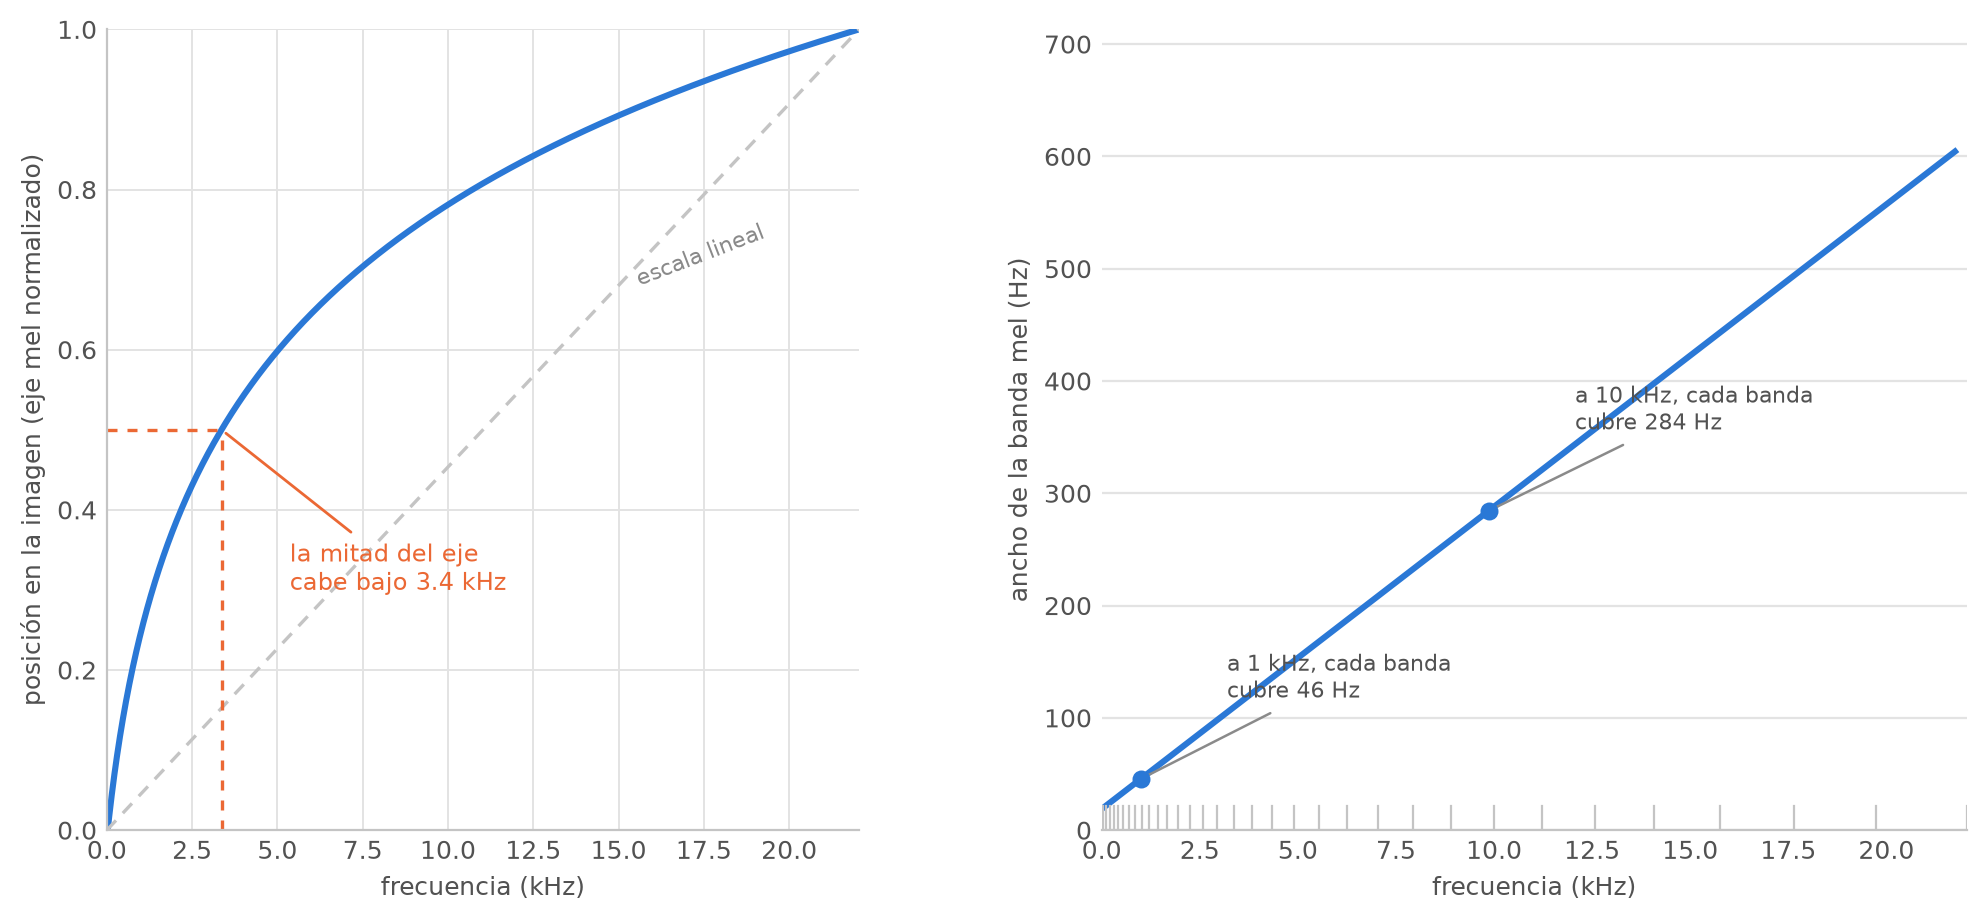
\includegraphics[width=\textwidth]{capitulos/02_marco_referencial/figures/mel_axis.png}
\end{figure}

La mitad del eje vertical queda por debajo de 3,4\,kHz, y el ancho de cada banda
crece con la frecuencia: 46\,Hz a 1\,kHz y 284\,Hz a 10\,kHz. Para este corpus la
consecuencia es concreta: las llamadas agudas, como las de los tamarinos, quedan
comprimidas en pocas bandas, y una caja de altura fija en el marco normalizado
cubre en los agudos una banda mucho más ancha que en los graves
(ecuación~\ref{eq:mel-inv}).

La elección de la representación no es un trámite. La compresión logarítmica no
es la única opción: la normalización de energía por canal (PCEN) combina control
adaptativo de ganancia y compresión de rango dinámico, y en detección
bioacústica de campo fue el contribuyente principal a la mejora de precisión
sobre la línea base log-mel \citep{lostanlen_robust_2019}. Su ventaja depende,
sin embargo, de una condición del ruido: proviene de estimar y descontar un fondo
que varía lentamente respecto de la escala temporal del evento. El coro de
insectos amazónico cumple esa condición, pues es cuasi-estacionario durante
minutos, pero la lluvia y las ráfagas de viento no la cumplen, y sobre ellas el
control de ganancia puede atenuar la propia vocalización junto con el fondo.

Esta tesis adopta el log-mel. El extractor de la arquitectura propuesta, el
\textit{Audio Spectrogram Transformer} (AST), se preentrenó sobre espectrogramas
log-mel \citep{gong_ast_2021}, y ese preentrenamiento solo se aprovecha si la
entrada conserva la misma representación; las líneas base, preentrenadas en
imágenes, reciben el mismo log-mel escalado como imagen. La
Figura~\ref{fig:frontends} muestra por qué la compresión es imprescindible:
pinta la misma ventana sin comprimir y en log-mel.

\begin{figure}[htbp]
    \centering
    \caption{Mel de potencia y log-mel sobre la misma ventana}
    \label{fig:frontends}
    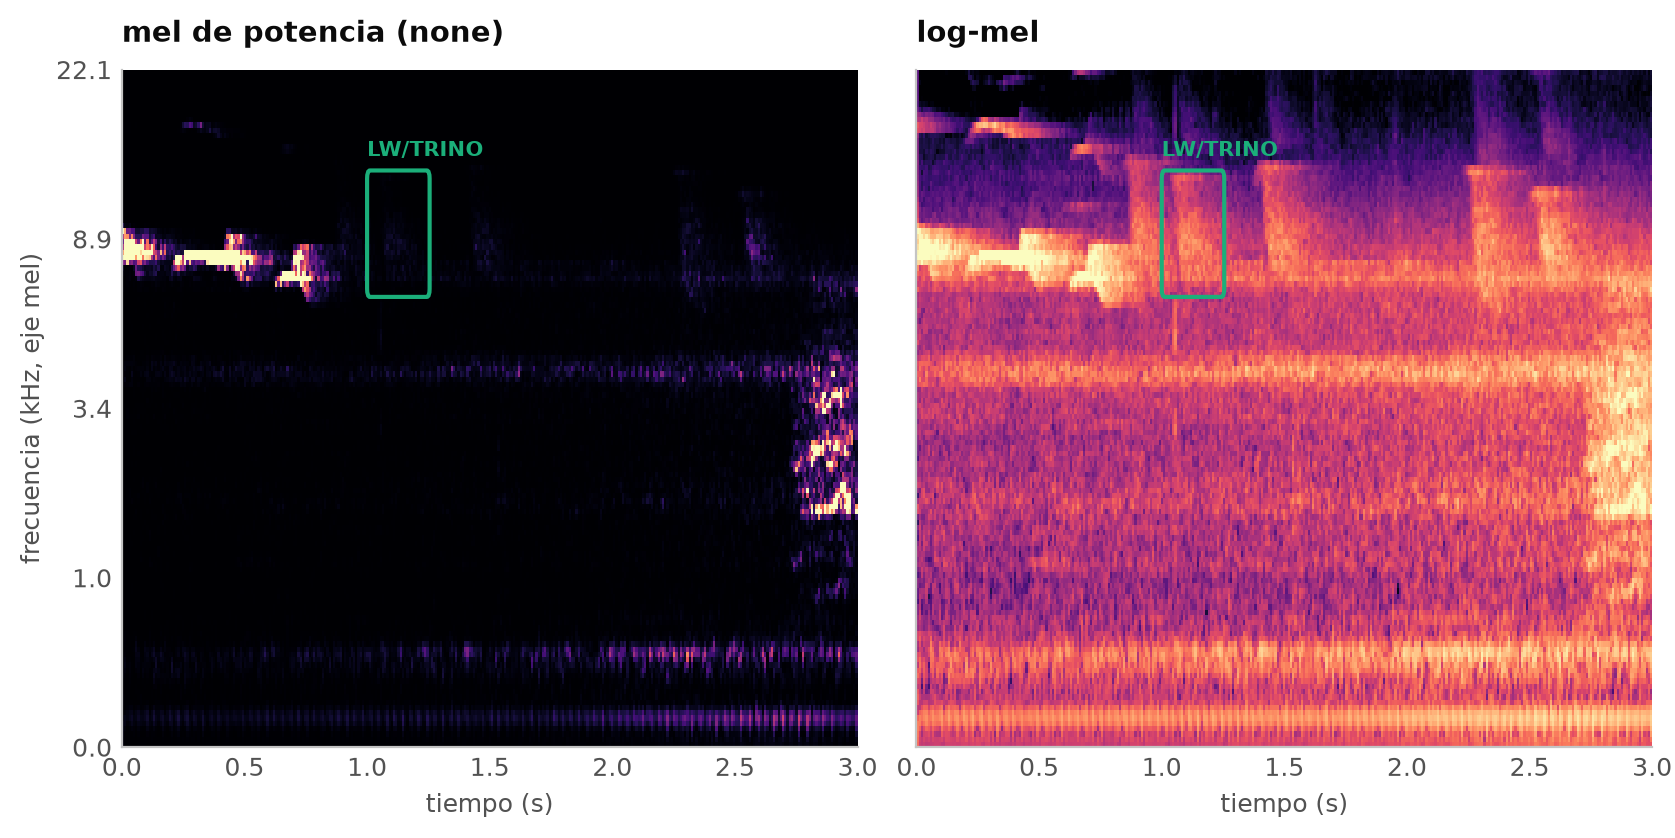
\includegraphics[width=\textwidth]{capitulos/02_marco_referencial/figures/frontends.png}
\end{figure}

La caja marca un trino del tamarino de Weddell (\texttt{LW/TRINO}). Sin
compresión, el mel de potencia solo muestra los sonidos más intensos y el trino
casi desaparece; el log-mel lo hace visible, pero también el coro de fondo, que
ocupa bandas enteras durante toda la ventana. Queda así una imagen en la que el
evento es visible; falta el mecanismo que lo localice dentro de ella.

\subsection{Detección de eventos sonoros}

La detección de eventos sonoros (SED) consiste en identificar la presencia de un
evento y localizar sus límites sobre la representación tiempo--frecuencia. La
distinción decisiva dentro de esta tarea es la \emph{forma de la salida}, con la
que la sección~\ref{sec:soluciones} ordenó las soluciones existentes
(Figura~\ref{fig:output-forms}). Expresada en los términos de la
ecuación~\eqref{eq:tupla}, la gradación es la siguiente: la salida por segmento
fijo cuantiza $t_{\text{ini}}$ y $t_{\text{fin}}$ al tamaño del segmento y no
estima la banda de frecuencia; la salida temporal estima $t_{\text{ini}}$ y
$t_{\text{fin}}$, pero descarta $f_{\min}$ y $f_{\max}$, que al tratar los eventos
acústicos se establecieron como magnitudes físicas del aparato fonador, y solo la
salida tiempo--frecuencia emite la tupla completa. Es la única que coincide con lo
que el analista produce a mano en Raven y, por tanto, la única que puede sustituir
su insumo en lugar de complementarlo. Esa propiedad explica por qué los
detectores existentes, que no emiten la tupla completa, no alivian la búsqueda que
describe la causa C2 del árbol de problemas.

El problema impone seis exigencias, y cada familia de la literatura responde a
una de ellas. Presentarlas en orden cronológico no dice nada; presentarlas por la
exigencia que satisfacen permite decidir, y así las ordena la
Tabla~\ref{tab:familias}. Las vocalizaciones de primates se organizan en
secuencias cuya identidad depende del orden y del espaciado de sus unidades, lo
que explica por qué el contexto largo aparece como exigencia propia y no como un
refinamiento del reconocimiento local.

\begin{table}[htbp]
    \centering
    \caption{Arquitecturas frente a requisitos}
    \label{tab:familias}
    \small
    \begin{tabular}{@{}L{4.0cm}L{3.4cm}L{7.2cm}@{}}
        \toprule
        \textbf{Exigencia}                                     & \textbf{Familia} & \textbf{Qué aporta y dónde se queda corta} \\
        \midrule
        Reconocer un patrón espectro-temporal local            &
        Redes convolucionales                                  &
        Aplican filtros sobre vecindades del espectrograma y reconocen patrones
        locales, pero por sí solas no sostienen el contexto de una secuencia ni
        emiten cajas                                                                                                           \\
        \addlinespace
        Sostener el contexto a lo largo de una frase           &
        Convolucionales recurrentes                            &
        Añaden capas recurrentes sobre las características convolucionales para
        sostener el contexto temporal; su salida sigue siendo una probabilidad por
        trama                                                                                                                  \\
        \addlinespace
        Ganar profundidad sin degradación                      &
        Conexiones residuales                                  &
        Permiten entrenar redes muy profundas sin pérdida de desempeño
        \citep{he_deep_2016}                                                                                                   \\
        \addlinespace
        Modelar dependencias a larga distancia sin recurrencia &
        Transformadores                                        &
        La autoatención relaciona en paralelo todas las posiciones del
        espectrograma; el \textit{Audio Spectrogram Transformer} lleva esa idea al
        audio, pero produce representaciones de una sola escala
        \citep{zhu_sound_2025}                                                                                                 \\
        \addlinespace
        Preservar la posición en frecuencia                    &
        Ninguna de las anteriores por sí sola                  &
        La convolución bidimensional estándar es equivariante a traslación en
        ambos ejes, propiedad deseable en tiempo y errónea en frecuencia;
        corregirlo exige adaptar el filtro a la banda \citep{nam_frequency_2022}                                               \\
        \addlinespace
        Emitir $f_{\min}$ y $f_{\max}$                         &
        Cabezas de detección de objetos                        &
        Única salida que coincide con la tupla de la ecuación~\eqref{eq:tupla};
        es la familia descrita en la sección~\ref{sec:objetos}                                                                 \\
        \bottomrule
    \end{tabular}
\end{table}

El criterio de descarte es la forma de la salida, no el desempeño reportado. Una
arquitectura solo es candidata a arquitectura final si su cabeza puede emitir
$f_{\min}$ y $f_{\max}$. Bajo esa regla, las cuatro primeras familias de la
Tabla~\ref{tab:familias} quedan descartadas \emph{como sistema
    completo}, porque su formulación habitual termina en una probabilidad por trama o
por segmento; ninguna queda descartada \emph{como extractor de características},
que es el papel en el que siguen siendo pertinentes. La cabeza que sí satisface
la exigencia es la de los detectores de objetos descritos en la
sección~\ref{sec:objetos}, y por eso la arquitectura de esta tesis combina un
extractor de audio con una cabeza de detección, en lugar de adoptar una de las
cuatro familias tal como se emplean en la literatura de SED.

Localizado el evento, queda el problema de nombrarlo.

\subsection{Clasificación jerárquica}
\label{sec:etiqueta}

La etiqueta que el analista necesita contiene dos niveles anidados,
la especie y, dentro de su repertorio, el tipo de llamada. Las unidades acústicas se agrupan en notas,
trinos, sílabas, frases, motivos y cantos, y pueden estar jerárquicamente anidadas:
una secuencia de unidades puede considerarse ella misma una unidad y ser reemplazada por una
etiqueta única \citep{kershenbaum_acoustic_2016}.

El primer nivel se define sobre las ocho especies de la
Tabla~\ref{tab:resumen-dataset}, identificadas por su código de dos letras.

El segundo nivel de la etiqueta se define dentro de cada especie, sobre el
vocabulario de la Tabla~\ref{tab:repertorio}. Los repertorios están desbalanceados, de modo que los 41
pares posibles no se reparten de forma pareja entre las ocho especies, y esa
asimetría es la que condiciona la elección del esquema de clasificación.

\begin{table}[htbp]
    \centering
    \small
    \begin{threeparttable}
        \caption{Repertorio por especie}
        \label{tab:repertorio}
        \begin{tabular}{@{}L{2.6cm}L{10.4cm}r@{}}
            \toprule
            \textbf{Especie}                               & \textbf{Tipos de llamada (código: nombre)} & \textbf{N.\textsuperscript{o}} \\
            \midrule
            AA \textit{Aotus azarae}                       &
            \texttt{gc}: \textit{gulp};
            \texttt{hm}: \textit{hoot};
            \texttt{sc}: \textit{squeak}                   & 3                                                                           \\
            \addlinespace
            AC \textit{Ateles chamek}                      &
            \texttt{chc}: \textit{chitter};
            \texttt{gc}: \textit{growl};
            \texttt{cc}: \textit{contact};
            \texttt{whc}: \textit{whinnie};
            \texttt{sc}: \textit{squeak};
            \texttt{bc}: \textit{bark}                     & 6                                                                           \\
            \addlinespace
            AS \textit{Alouatta sara}                      &
            \texttt{hc}: \textit{howl};
            \texttt{bc}: \textit{bark}                     & 2                                                                           \\
            \addlinespace
            CC \textit{Cebus cuscinus}                     &
            \texttt{cc}: \textit{contact}                  & 1                                                                           \\
            \addlinespace
            LW \textit{Leontocebus weddelli}               &
            \texttt{cc}: \textit{contact};
            \texttt{cs}: \textit{contact syllable};
            \texttt{aa}: \textit{aerial alarm};
            \texttt{ta}: \textit{terrestrial alarm};
            \texttt{sqc}: \textit{squeal};
            \texttt{phc}: \textit{phee};
            \texttt{tr}: \textit{trino};
            \texttt{tf}: \textit{trino fast};
            \texttt{tt}: \textit{trino transition};
            \texttt{tj}\tnote{$\dagger$}: sin denominación;
            \texttt{vc}: \textit{visual contact}           & 11                                                                          \\
            \addlinespace
            PT \textit{Plecturocebus toppini}              &
            \texttt{dc}: \textit{duet};
            \texttt{ac}: \textit{alarm};
            \texttt{bp}\tnote{$\dagger$}: \textit{bellow phrase};
            \texttt{pp}\tnote{$\dagger$}: \textit{pant phrase};
            \texttt{sqc}\tnote{$\dagger$}: \textit{squeal} & 5                                                                           \\
            \addlinespace
            SB \textit{Saimiri boliviensis}                &
            \texttt{pcc}: \textit{peep contact};
            \texttt{ppc}: \textit{play peep};
            \texttt{lpc}: \textit{long peep};
            \texttt{spc}: \textit{spit};
            \texttt{sc}: \textit{shriek}                   & 5                                                                           \\
            \addlinespace
            SM \textit{Sapajus macrocephalus}              &
            \texttt{cc}: \textit{contact};
            \texttt{acc}: \textit{aggressive contact};
            \texttt{sc}: \textit{squeal};
            \texttt{pc}: \textit{purr};
            \texttt{whc}: \textit{whistle};
            \texttt{hic}: \textit{hip};
            \texttt{fc}: \textit{food};
            \texttt{fs}: \textit{food syllable}            & 8                                                                           \\
            \midrule
            \textbf{Total}                                 &                                            & \textbf{41}                    \\
            \bottomrule
        \end{tabular}
        \begin{tablenotes}[flushleft]
            \footnotesize
            \item[$\dagger$] Categorías sin nombre establecido en la literatura
            del repertorio, acuñadas por el equipo de anotación. El
            Capítulo~\ref{cap:curacion} documenta cuáles de ellas sobreviven al
            vocabulario cerrado y cuáles se descartan por ser unidades de nivel
            de frase.
        \end{tablenotes}
    \end{threeparttable}
\end{table}

Un mismo código puede designar llamadas distintas en especies distintas:
\texttt{sc} es \textit{squeak} en AA y AC, \textit{shriek} en SB y
\textit{squeal} en SM. Por eso la unidad de etiquetado en el resto del documento
es siempre el par, escrito \texttt{especie/tipo}, y nunca el código de llamada
por sí solo.

Ante esa estructura caben tres esquemas. La \emph{clasificación plana} crea una
clase por cada par y trata la jerarquía como inexistente. El enfoque \emph{local
    por nodo padre} entrena un clasificador de especie y, debajo, un clasificador de
tipo por cada especie. El \emph{modelo global jerárquico} aprende la estructura
completa de una vez. Esta tesis adopta la clasificación plana sobre un
vocabulario cerrado de pares: los esquemas jerárquicos exigen un número mínimo de
ejemplos en cada nodo hijo, y el desbalance del corpus deja varios pares con
demasiados pocos como para sostener un clasificador propio. El
Capítulo~\ref{cap:curacion} documenta esa composición y cierra el vocabulario en
consecuencia.

Queda un supuesto implícito en todo lo anterior: que la etiqueta de referencia
contra la cual se entrena y se mide es un dato fijo. No lo es.

\subsection{Anotaciones inconsistentes}

Un sistema supervisado se entrena y se evalúa contra anotaciones humanas, de modo
que las propiedades de esas anotaciones forman parte del planteamiento y no del
apartado de limitaciones. Tres conceptos las describen.

\rotulo{Etiqueta fuerte y etiqueta débil.} Una etiqueta \emph{débil} declara que
una clase está presente en algún lugar de la grabación, sin decir dónde; es lo
que ofrecen los repositorios grandes de audio de fauna. Una etiqueta
\emph{fuerte} delimita el evento: aporta sus fronteras además de su clase. El
material de esta tesis es de etiqueta fuerte y bidimensional, pues delimita también
en frecuencia, lo que lo hace más informativo y, a la vez, más costoso de
producir y más expuesto a desacuerdo, porque hay más decisiones que tomar por
evento.

\rotulo{Acuerdo entre anotadores y consigo mismo.} El acuerdo
\emph{inter-anotador} mide cuánto coinciden dos analistas que anotan el mismo
audio; el \emph{intra-anotador}, cuánto coincide un mismo analista consigo mismo
al anotar dos veces el mismo segmento. Ambos son bajos en bioacústica, con las
magnitudes que reunió el análisis de la causa C1 (sección~\ref{sec:causas}).

\rotulo{Frontera borrosa del evento.} El desacuerdo anterior no se reparte de
forma uniforme: se concentra en los bordes. Una vocalización no empieza ni
termina en un instante definido, sino que emerge del fondo y se desvanece en él,
y lo mismo ocurre en frecuencia con los armónicos superiores. En detección de
cajas tiempo--frecuencia se observan desplazamientos relativamente grandes entre
la caja predicha y la anotada, de lo que se concluye que las fronteras de los
eventos son borrosas y difíciles de determinar \citep{zhu_sound_2025}.

Estos tres conceptos dan forma conceptual a la causa C1 del árbol de problemas:
a la heterogeneidad de las anotaciones y a la referencia incompleta que impide
medir los errores sin un especialista. También fundamentan
las dos decisiones de evaluación que fijó la sección~\ref{sec:metricas}: emparejar
con un IoU bajo evita medir el acuerdo con un borde que el propio anotador no
reproduce, y priorizar el \textit{recall} evita descartar como error lo que puede
ser un evento válido ausente de una referencia incompleta.

% ===================================================================
% CAPÍTULO 3
% ===================================================================
